\begin{figure*}
\begin{subfigure}{0.24\textwidth}
\centering
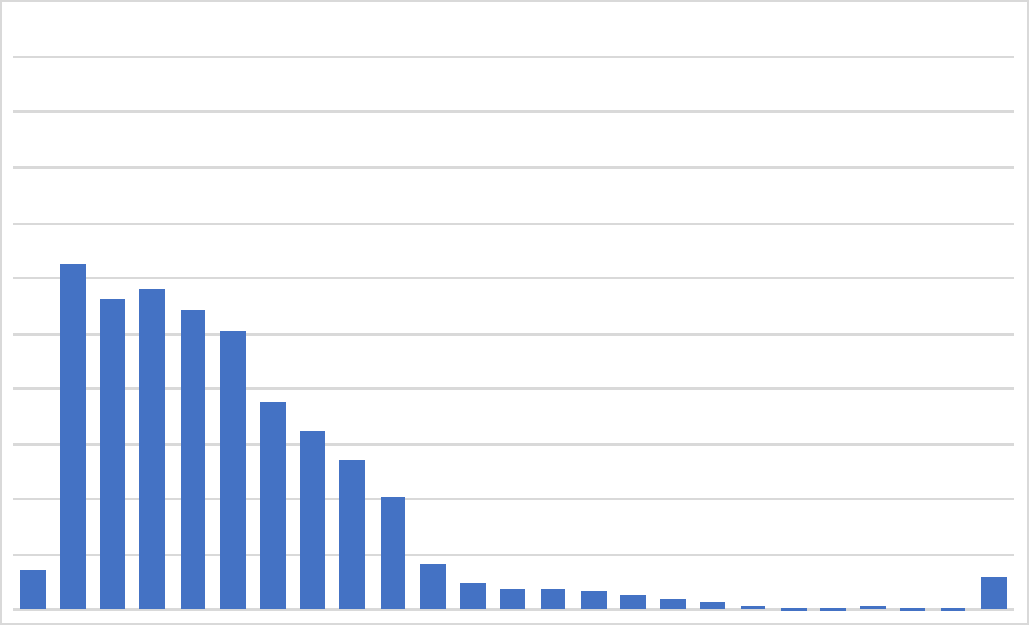
\includegraphics[width=0.7\linewidth]{results/sw4/Eul1_AvgL2.pdf}
\caption{Eulerian 250 Avg$_{L2}$}
\end{subfigure}
\begin{subfigure}{0.24\textwidth}
\centering
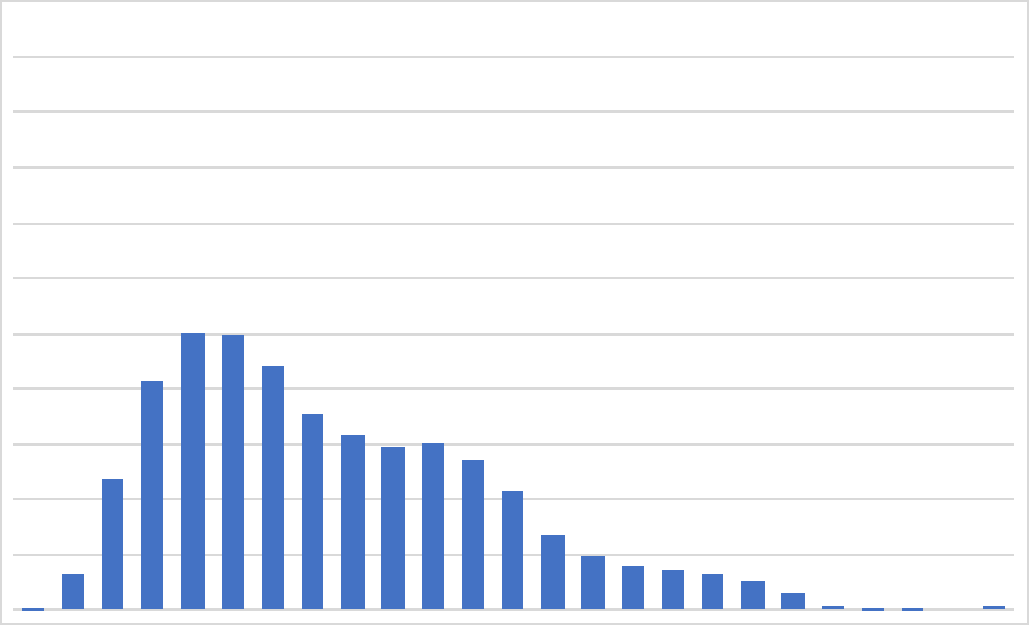
\includegraphics[width=0.7\linewidth]{results/sw4/Eul2_AvgL2.pdf}
\caption{Eulerian 500 Avg$_{L2}$}
\end{subfigure}
\begin{subfigure}{0.24\textwidth}
\centering
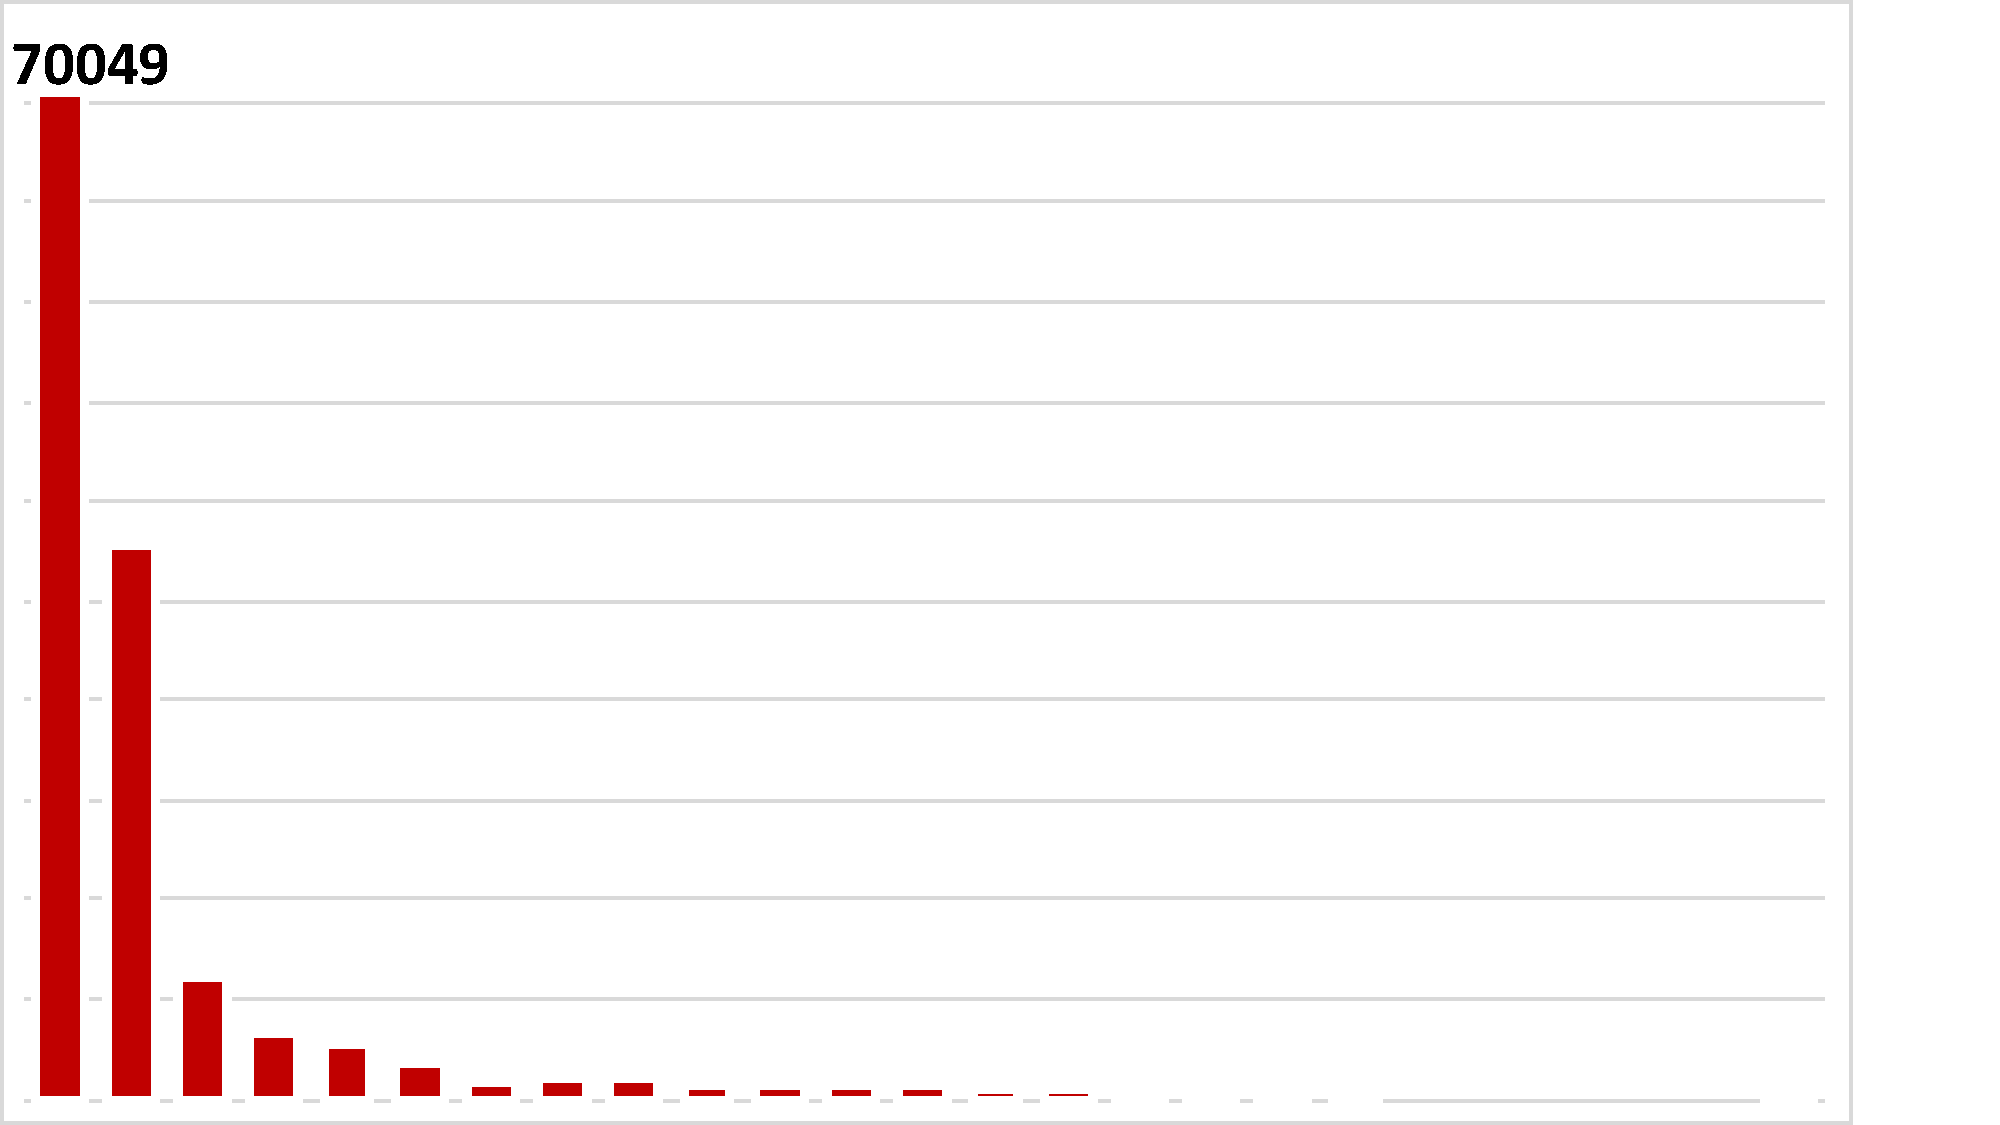
\includegraphics[width=0.8\linewidth]{results/sw4/Lag3_AvgL2.pdf}
\caption{Lagrangian 250 1:27 Avg$_{L2}$}
\end{subfigure}
\begin{subfigure}{0.24\textwidth}
\centering
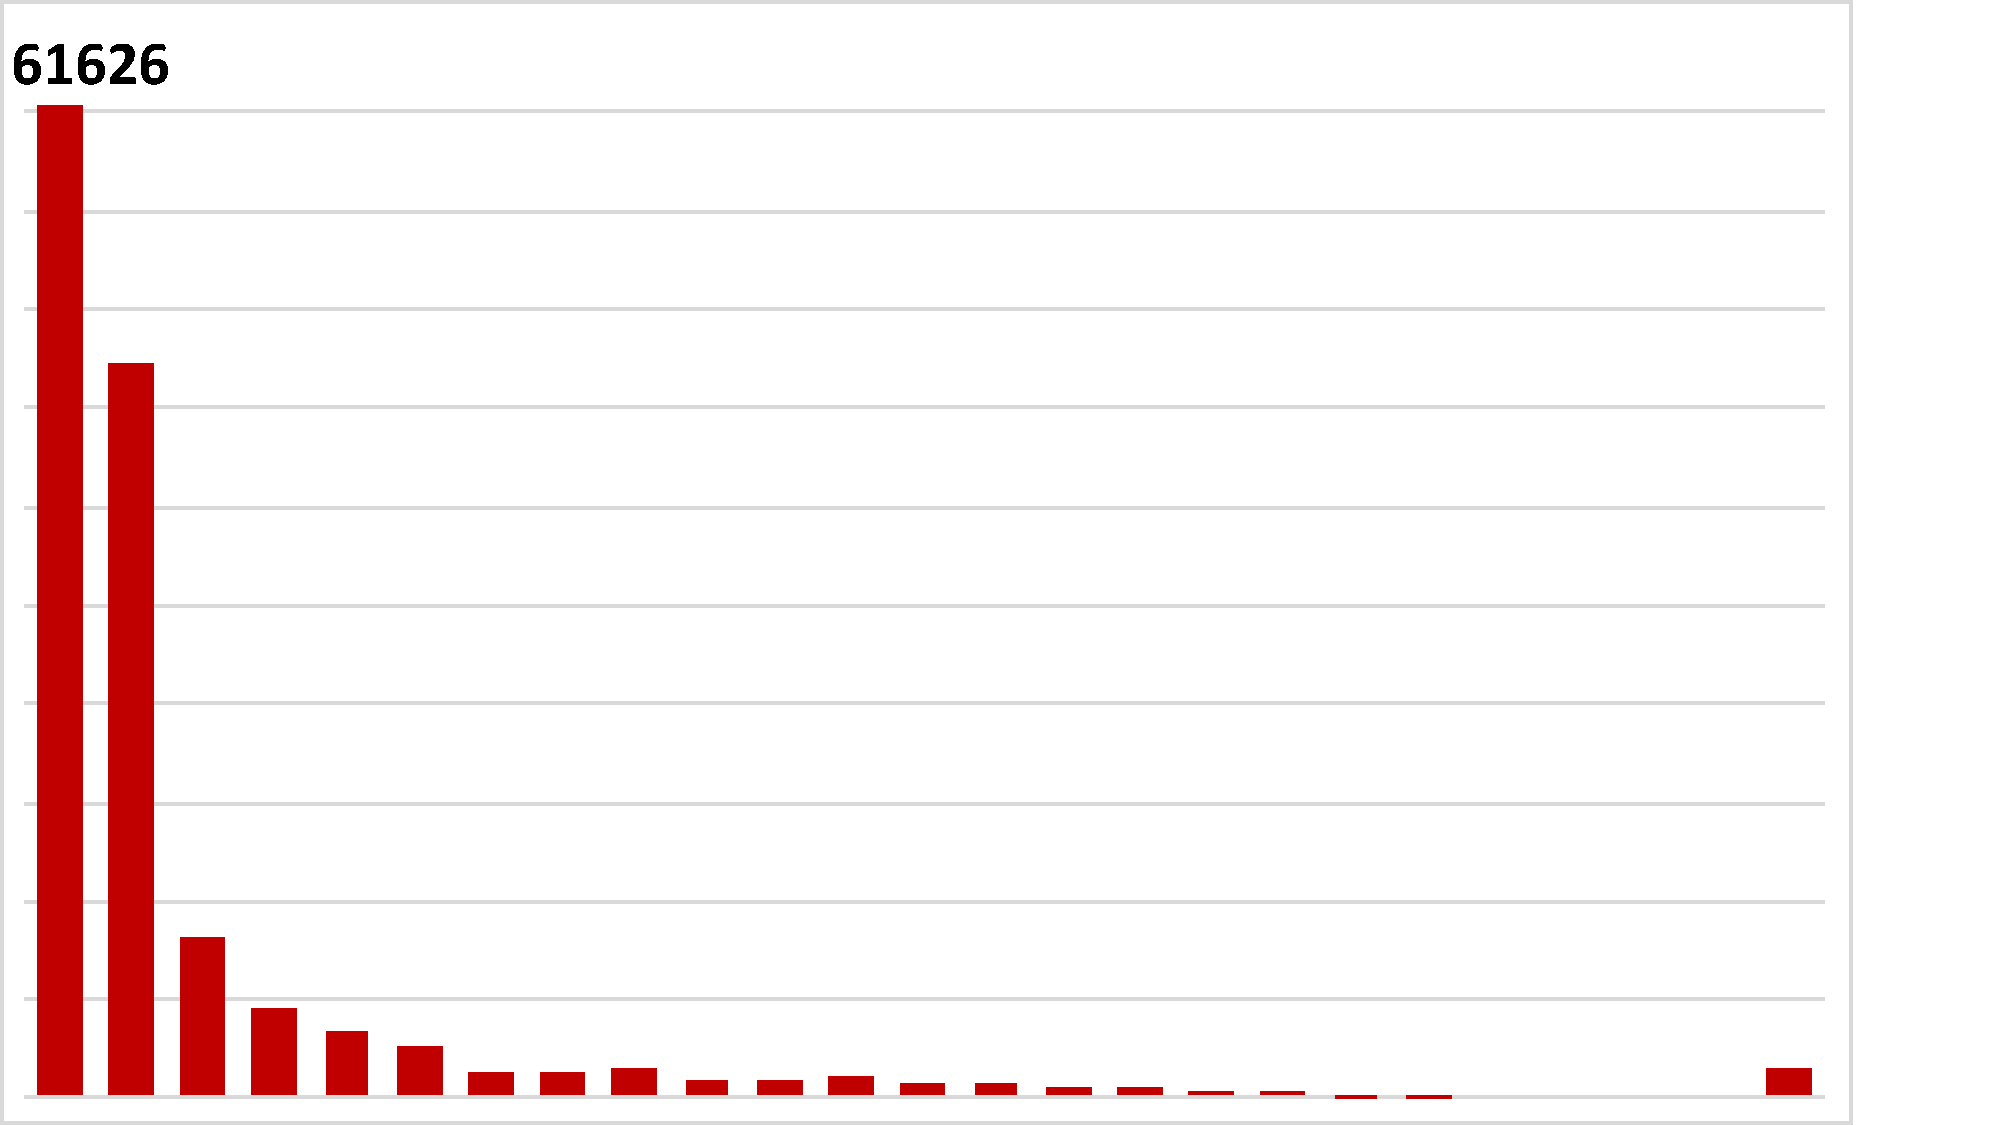
\includegraphics[width=0.8\linewidth]{results/sw4/Lag4_AvgL2.pdf}
\caption{Lagrangian 250 1:64 Avg$_{L2}$}
\end{subfigure}
\begin{subfigure}{0.24\textwidth}
\centering
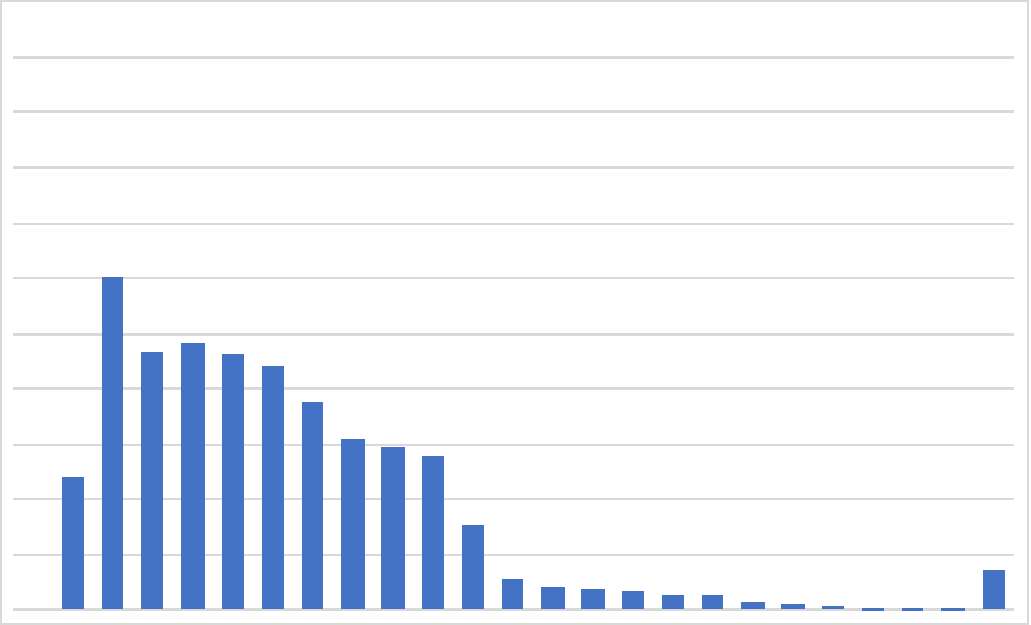
\includegraphics[width=0.7\linewidth]{results/sw4/Eul1_Max.pdf}
\caption{Eulerian 250 Max$_{L2}$}
\end{subfigure}
\hspace{1mm}
\begin{subfigure}{0.24\textwidth}
\centering
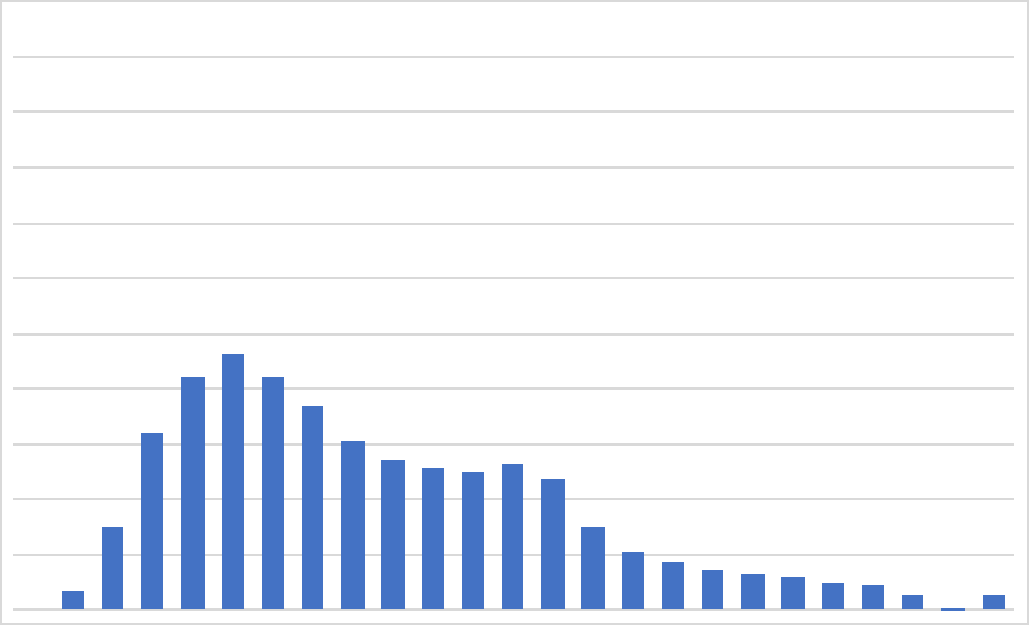
\includegraphics[width=0.7\linewidth]{results/sw4/Eul2_Max.pdf}
\caption{Eulerian 500 Max$_{L2}$}
\end{subfigure}
\hspace{1mm}
\begin{subfigure}{0.24\textwidth}
\centering
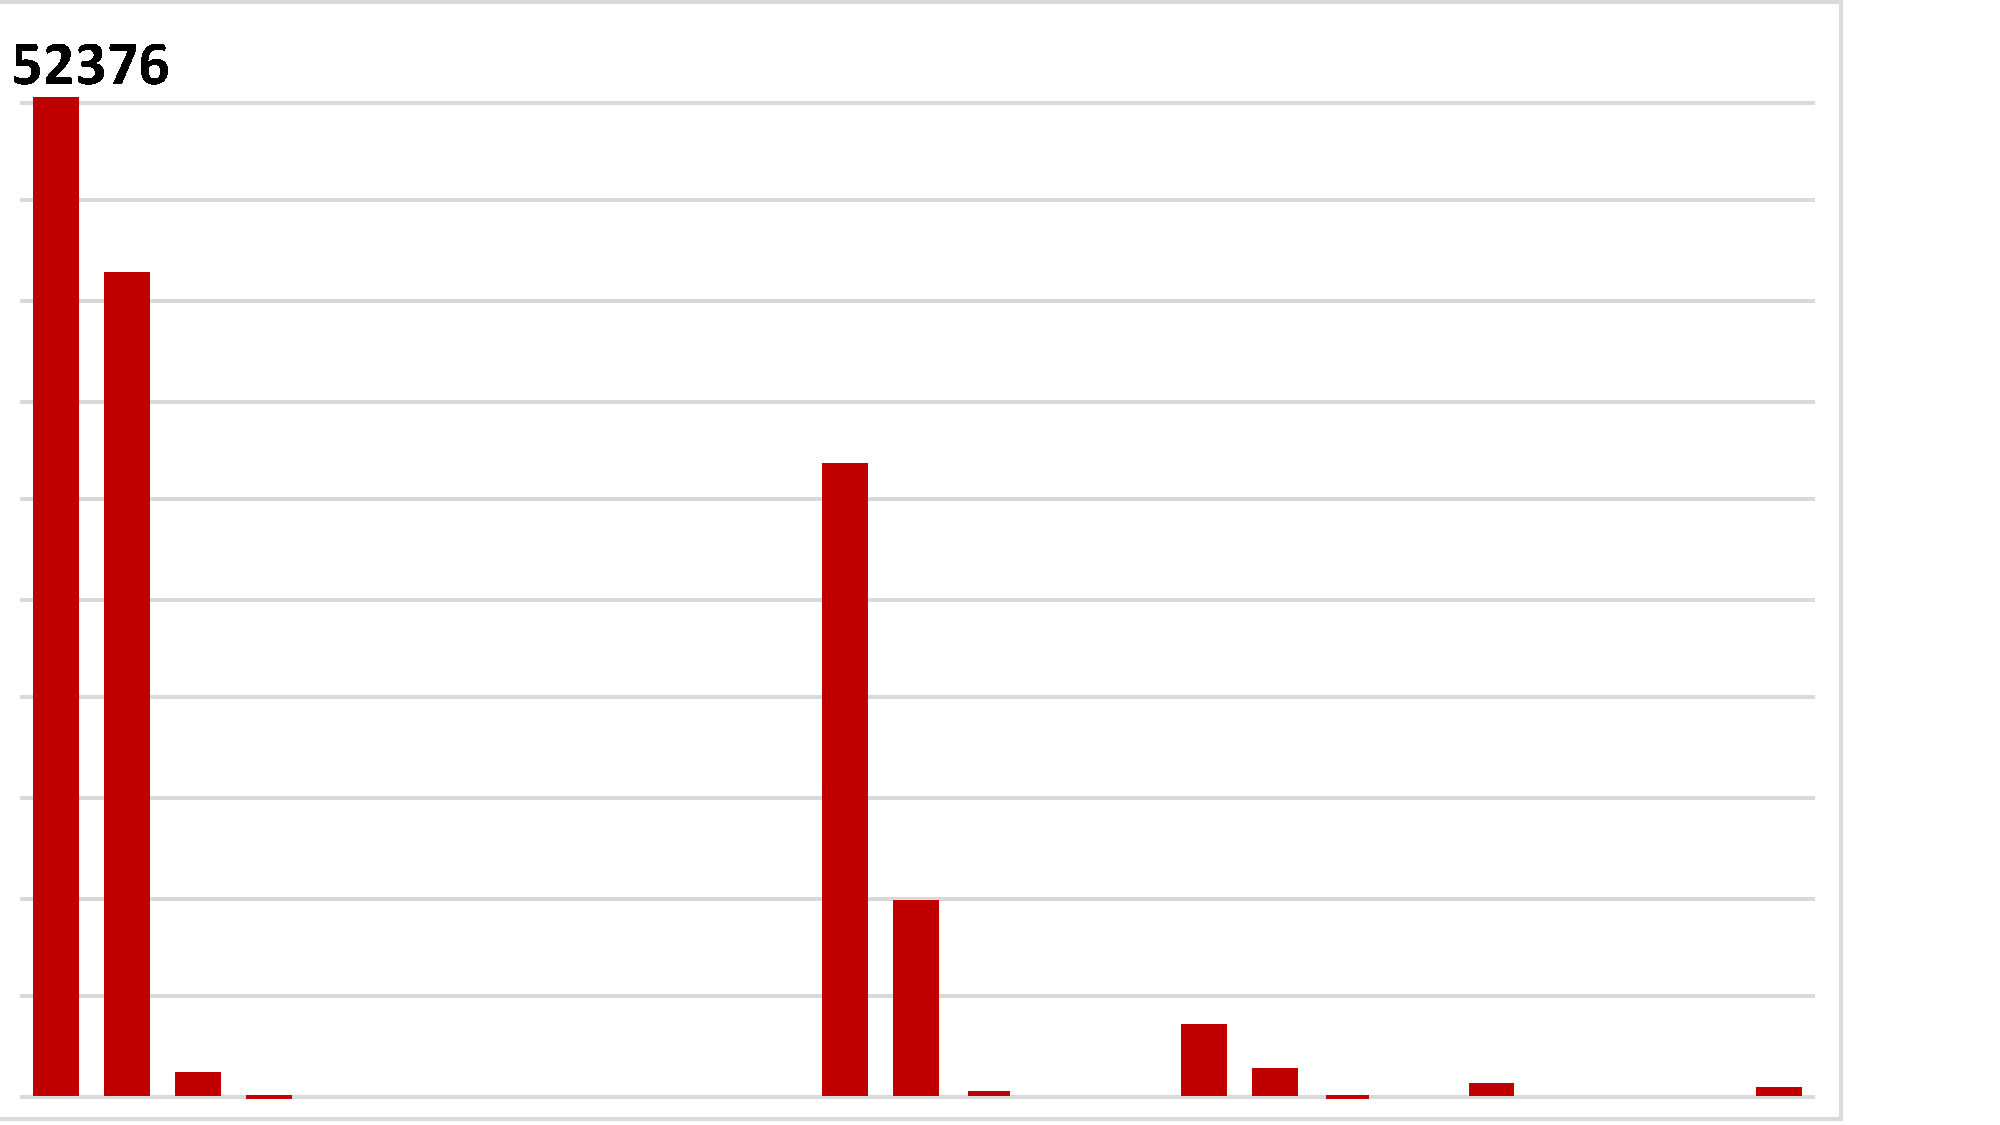
\includegraphics[width=0.8\linewidth]{results/sw4/Lag3_Max.pdf}
\caption{Lagrangian 250 1:27 Max$_{L2}$}
\end{subfigure}
\hspace{1mm}
\begin{subfigure}{0.24\textwidth}
\centering
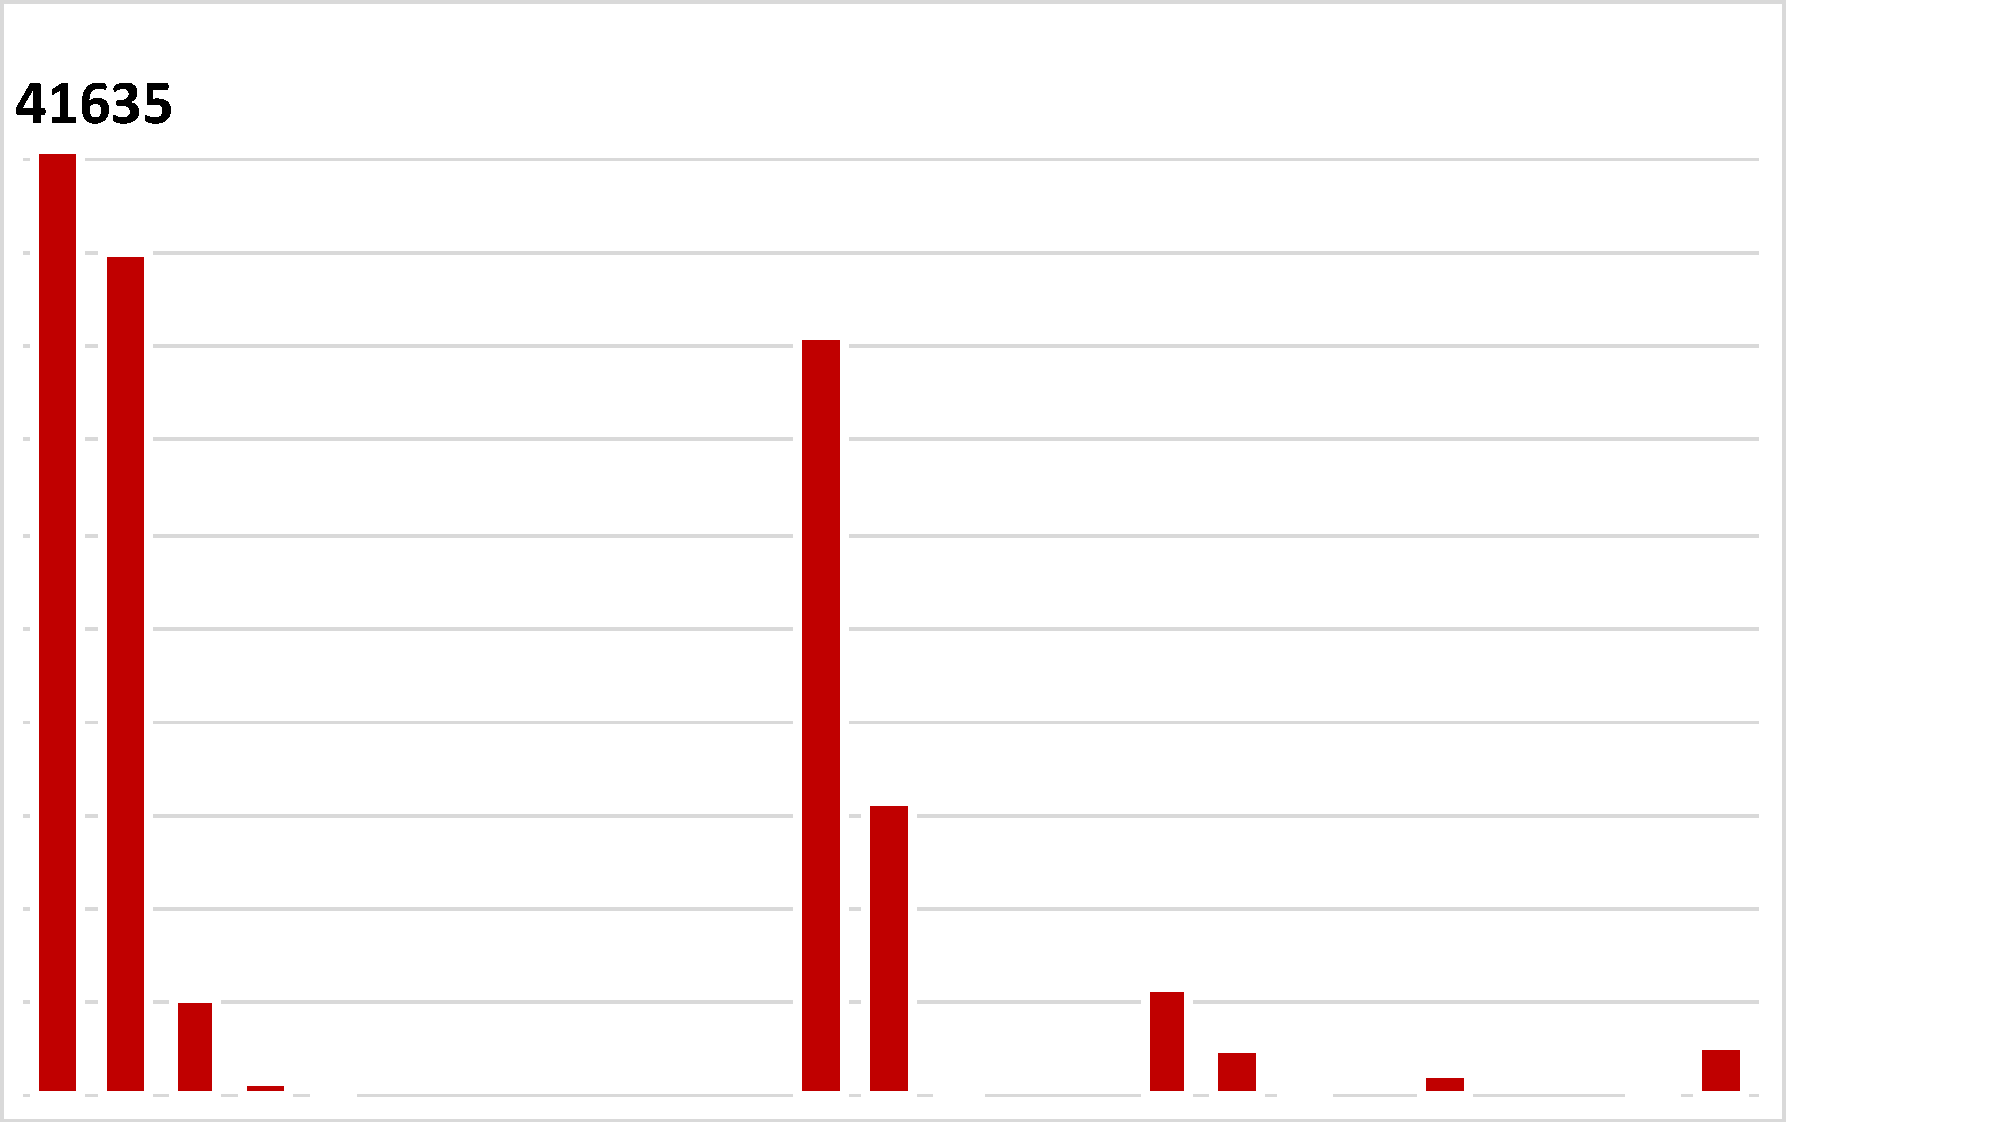
\includegraphics[width=0.8\linewidth]{results/sw4/Lag4_Max.pdf}
\caption{Lagrangian 250 1:64 Max$_{L2}$}
\end{subfigure}
\caption{SW4 experiment histograms for 90,000 test particle interpolation errors. Each plot has 25 bins, Eulerian bins range from $<$0.6 to $>$15, Lagrangian bins range from 0 to $>$0.2, with bar height encoding number of particles. Horizontal grid lines mark increments of 2,000.}
\label{fig:sw4_histograms}
\end{figure*}

